\section{Introduction}
\subsection{History of Argumentation Theory}
\par
Argumentation has its roots in Ancient Greece, where the art of rhetoric developed first. Aristotle defines the rhetorician as someone who is always able to see what is persuasive. Correspondingly, rhetoric is defined as the ability to see what is possibly persuasive in every given case.  Argumentation theorists have searched for the requirements that make an argument correct, by some appropriate standard of proof, by examining the errors of reasoning we make when we try to use arguments. These errors have been called fallacies. Until the 1950s, the approach of argumentation was based on rhetoric and logic.
\par
In 1895, George Pierce Baker writes ``The Principles of Argumentation'' giving the following definition: ``Argumentation is the art of producing in the mind of someone else a belief in the ideas which the speaker or writer wishes the hearer or reader to accept''. In the United States debating and argumentation became an important subject on universities and colleges. In the 1960s and 1970s Perelman and Toulmin were the two of the most influential writers on argumentation. Perelman tried to find a description of techniques of argumentation used by people to obtain the approval of others for their opinions. Perelman called this `new rhetoric. Toulmin developed his theory (starting in 1950s) in order to explain how argumentation occurs in the natural process of an everyday argument. He called his theory `The uses of Argument`. 
\par
Hamblin took, as well, a radical approach to argumentation. Considering the fact that deductive logic did not seem to be enough, Hamblin proposed a new concept for describing arguments: he considered it not just as an arbitrarily designated set of propositions, but as a move one party makes in a dialog to offer premises that may be acceptable to another party who doubts the conclusion of the argument.
Hamblin and Perelman's work announced a new field of study: informal logic. Nowadays,  research in informal logic increasingly incorporates the approaches to argumentation found in cognate disciplines and fields like Speech Communication, Rhetoric, Linguistics, Artificial Intelligence, Cognitive Psychology and Computational Modeling. Looked at from this perspective, informal logic as a discipline is an integral part of a much broader multi-disciplinary attempt to develop an ``argumentation theory'' that can account for informal reasoning.

\subsection{Argumentation in Computer Science}
\par
With regards to computer science, the study of argumentation is crucial in many artificial intelligence and natural language research problems.
\par
For example, in the field of Multi Agent Systems (MAS) reasoning agents need to communicate with each other and apply argumentation-based reasoning mechanisms to resolve the conflicts arising from their different views of goals, beliefs, and actions. Another example are question answering systems, which deal with finding the correct response to questions like ``Why was this decision taken?'' and therefore integrate the analysis of argumentation as a crucial part of identifying the answer to the questions as well as the pros and cons that make up the answer.
\par
The field of computer-supported collaborative learning (CSCL) has, in particular, been interested in argumentation and how students can benefit from it\cite{steg1}. So-called ``collaborative argumentation'' is viewed as a key way in which students can learn critical thinking, elaboration, and reasoning. Therefore, it is a crucial point to understand the characteristics and models of argumentation.
\par
Some relevant work in this area has been done by R.M. Palau and M-F Moens in\cite{palau1}\cite{palau2}. In these papers they analyze the main research questions when dealing with argumentation mining and the different methods they have studied and developed in order to successfully confront the challenges of argumentation mining in legal texts.
A different approach is taken by Safia ABBAS and Hajime SAWAMURA in\cite{safia}.  Their environment uses different mining techniques to manage a highly structured arguments repository.
\par
This area of natural language processing also lacks corpora resources. In our knowledge there are only two corpora used extensively in argumentation research, the \textit{Araucaria}\cite{araucaria}\cite{reed1} developed by Chris Reed and Glenn Glove in the Argumentation Research Group at University of Dundee and \textit{HUDOC} developed by the European Court of Human Rights\cite{echr}. Below is a summary of the structure of these two corpus:
\begin{table}[tbh]
\caption{Structure of arguments in ECHR and Araucaria}
\centering
\begin{tabular}{|c |c |c|}
\hline
Characteristics & ECHR & Araucaria \\
\hline
Number of documents & 47 & 641 \\
Number of arguments & 257 & 641 \\
Number of words & 92190 & 76970 \\
Number of sentences & 2571 & 3798 \\
\hline
\end{tabular}
\label{tab:eas}
\end{table}
\par
Overall, the task of argument extraction from free text is a new and difficult research area, one that will hopefully see a lot of activity in the near future, because the results that can be obtained will be of great use in many related fields of natural language processing.

\section{Argumentation Concepts Overview}
\par A nice overview on argumentation tasks and concepts was given by Douglas Walton in his research reports\cite{ara1}. The next sections are inspired by his work.

\subsection{Main problems}
\par
There are four tasks undertaken by argumentation:
\begin{description}
\item Identification which means finding the premises and conclusion of arguments in a text and fitting that argument in an argumentation scheme;
\item Analysis which involves the identification of implicit premises or conclusion of arguments (such an argument is called an enthymeme);
\item Evaluation where the strength of an argument must be determined using a general criteria;
\item Invention which means constructing new arguments that can be used to prove some conclusion
\end{description}

\subsection{Argument definition}
\par
An argument is a set of statements (propositions), made up of three parts, a conclusion, a set of premises and inference from the premises to the conclusion. An argument can be supported by other arguments, or it can be attacked by other arguments, and by raising critical questions about it.
\par
The definition of `argument` relied on so far could be called a minimal inferential definition, and the method of argument diagramming shown so far fits this minimal definition. The boxes represent propositions and the arrows represent inferences from some propositions to others.
\par
The general approach or methodology of argumentation can be described as distinctively different from the traditional approach based on deductive logic. The traditional approach concentrated on a single inference, where the premises and conclusion are designated in advance, and applied formal models like propositional
calculus and quantification theory determine whether the conclusion conclusively follows from the premises. This approach is often called mono-logical.
\par
In contrast, the argumentation approach is called dialogical (or dialectical) in that it looks at two sides of an argument, the pro and the contrary. According to this approach, the method of evaluation is to examine how the strongest arguments for and against a particular proposition at issue interact with each other, and in particular how each argument is subject to probing critical questioning that reveals doubts about it. By this dialog process of pitting the one argument against the other, the weaknesses in each argument are revealed, and it is shown which of the two arguments is the stronger.
\subsection{Argument Attack and Refutation}
\par
There are several ways to attack an argument and the easiest way is to ask an appropriate critical question that raises doubt about the acceptability of the argument. When this happens, the argument temporarily defaults until the proponent can respond appropriately to the critical question. Another way to attack an argument is to question one of the premises. A third way to attack an argument is to put forward counter-argument that opposes the original argument, meaning that the conclusion of the opposing argument is the opposite (negation) of the conclusion of the original argument.
\par
A simple way to represent a sequence of argumentation is using a directed graph:
\begin{center}
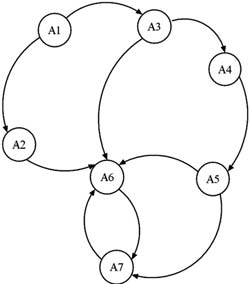
\includegraphics{attack.png}
\end{center}
\subsection{Argumentation Schemes}
\par
Some of the most common schemes are: argument from witness testimony, argument from expert opinion, argument from popular opinion, argument from example, argument from analogy, practical reasoning (from goal to action), argument from verbal classification, argument from sign, argument from sunk costs, argument from appearance, argument from ignorance, argument from cause to effect, abductive reasoning, argument from consequences, argument from alternatives, argument from pity, argument from commitment, ad hominem argument,argument from bias, slippery slope argument, and argument from precedent. Each scheme has a set of critical questions matching the scheme and such a set represents standard ways of critically probing into an argument to find aspects of it that are open criticism.
\subsection{Types of dialog}
There are six types of dialogs:
\begin{description}
\item[Persuasion] generated by a \textbf{Conflict of Opinions} in which each party tries to \textbf{Persuade Other Party} in order to \textbf{Resolve or Clarify Issue}
\item[Inquiry] generated by the \textbf{Need to Have Proof} in which each party tries to \textbf{Find and Verify Evidence} in order to \textbf{Prove (Disprove) the Hypothesis}
\item[Negotiation] generated by a \textbf{Conflict of Interests} in which each party tries to \textbf{Get What He Most Wants} in order to reach a \textbf{Reasonable Settlement Both Can Live With}
\item[Information-Seeking] catalyze by the \textbf{Need of Information} in which each party \textbf{Acquires or Gives Information} in order to \textbf{Exchange Information}
\item[Deliberation] generated by a \textbf{Deliberation Dilemma or Practical Choice} that is needed in which the participants try to \textbf{Co-ordinate Goals and Actions} in order to \textbf{Decide on Best Available Course of Action}
\item[Eristic] generated by a \textbf{Personal Conflict} in which each party tries to \textbf{Verbally Hit Out at Opponent} in order to \textbf{Reveal Deeper Basis of Conflict}.
\par
On our project we will focus on inquiry dialogs.
\end{description}
\subsection{Argumentation in Multi Agent Systems}
\par
Argumentation systems is a domain with large applications in industry, especially in e-commerce transactions, asset market and e-negotiation. Argumentation based dialogues have proved to be a general approach to agent communication in which the agents exchange not only statements of what they believe and what they want but also the reasons why. There is some research made in the field and several abstract argumentation frameworks were proposed\cite{amgoud}\cite{parsons}.
\par
We have designed a system that supports domain based argumentation. Each agent participating in a conversation has a knowledge base supported by one or more ontologies specific to a domain. This allows specialization of agents in a society.
